\cleardoublepage

\chapter{Initial Work}
\label{ch:initial_work}

\par In this chapter a fundamental tool used was imageAI, which is a Computer Vision Python library that allows developers the ability to easily use state-of-the-art AI features . It supports algorithms for image prediction, custom image prediction, object detection, video detection, video object tracking and image predictions trainings. ImageAI also supports object detection, video detection and object tracking using RetinaNet, YOLOv3 and TinyYOLOv3 trained on COCO dataset. In terms of Machine Learning algorithms imageAI supports 4 trained on the imageNet-1000 dataset. \cite{ImageAI}


\par With the goal of finding the best performing neural network or algorithm for image recognition and for object detection a few test runs were made. These test runs consist on feeding each of the neural networks and algorithms available for image recognition and object detection with one picture manually chosen beforehand. Each neural network and algorithm makes five guesses on what the image represents with a prediction probability that ranges in an interval between [0,100]. This prediction probability represents the certainty of the neural network and algorithm in its guess.
\par In sections \ref{sec:image_test} and \ref{sec:object_test} an overview of three example test runs are presented and analysed.



\section{Image Recognition test runs}
\label{sec:image_test}

\par The imageAI library allows the usage of 4 deep learning neural networks for image recognition which are DenseNet, inceptionV3, ResNet50, and SquezeeNet. The explanation on how these neural networks function is presented in chapter \ref{ch:computervision}. The analysis of the results is in section  \ref{sec:results_image_rec}



    \newpage
    \subsection{Test Run Number 1}

    \par For the first run an image of a dog (breed saluki) was analysed by all 4 neural networks.

    \begin{figure}[htb]
        \centering
        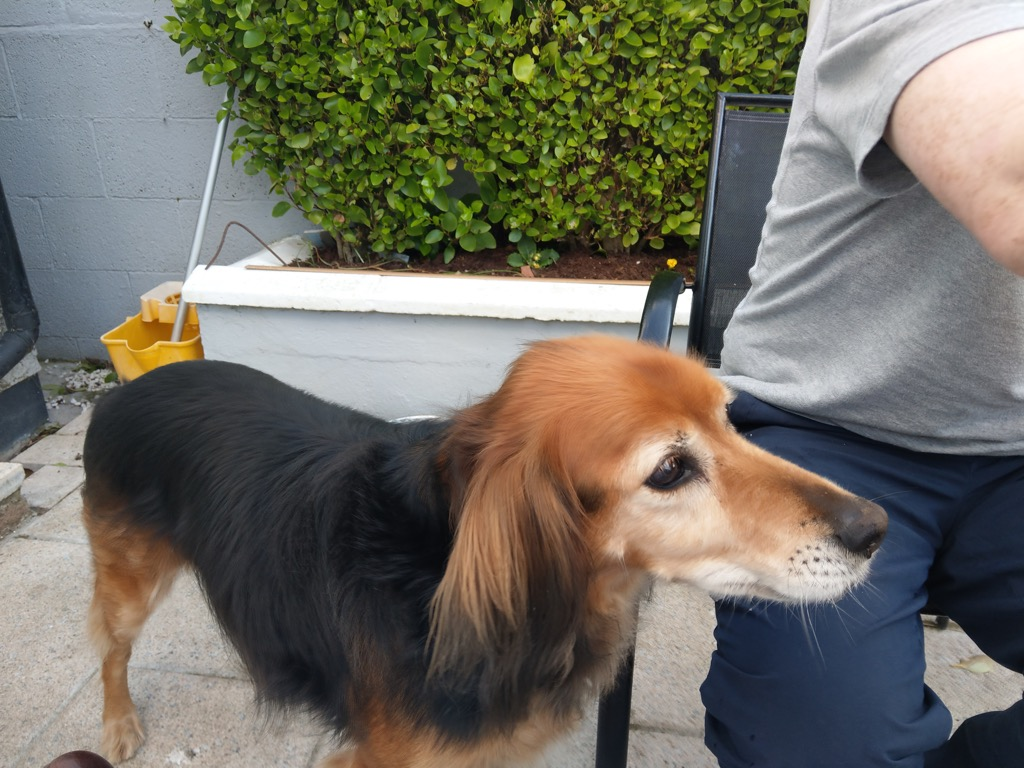
\includegraphics[scale = 0.20]{Sections/4InitialWork/4_images/run1_pic.jpg}
        \caption{First picture to be analysed.} 
    \end{figure}

    \par The obtained results can be seen in the figure below. 

    \begin{figure}[htb]
        \centering
        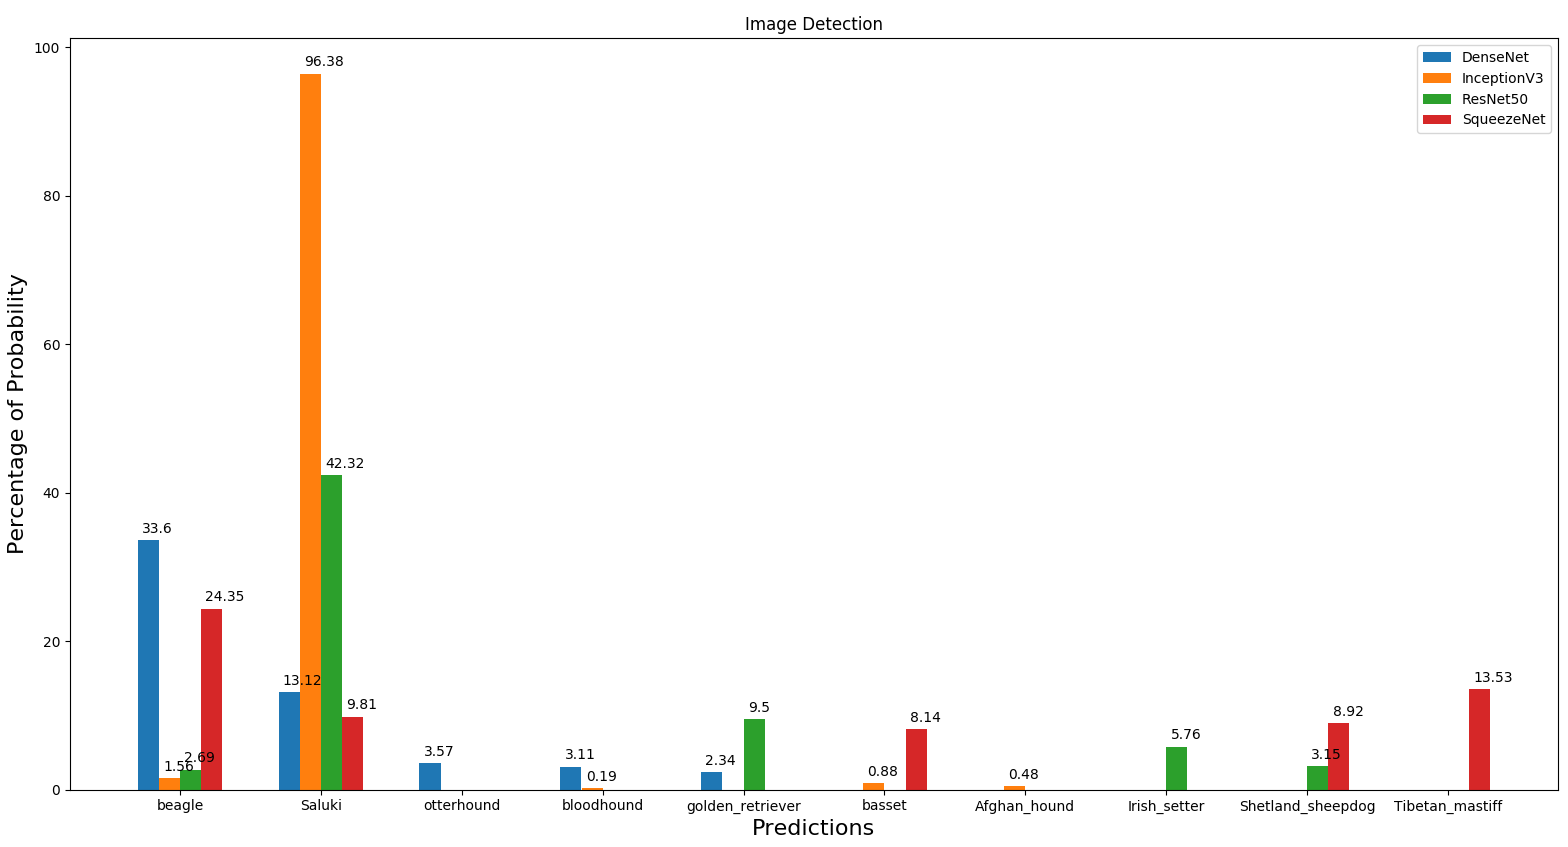
\includegraphics[scale = 0.37]{Sections/4InitialWork/4_images/run1_res.png}
        \caption{Results obtained.} 
    \end{figure}


    \newpage
    \subsection{Test Run Number 2}
    \par For the second run an image of a car was analysed by all 4 neural networks.

    \begin{figure}[htb]
        \centering
        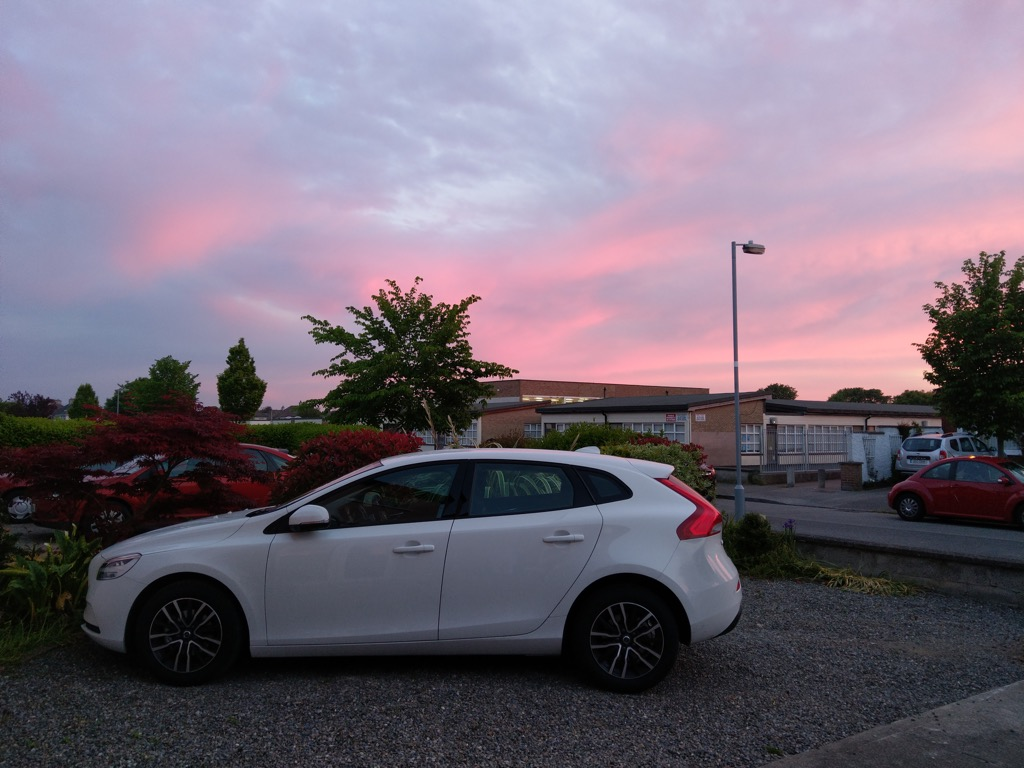
\includegraphics[scale = 0.2]{Sections/4InitialWork/4_images/run3_pic.jpg}
        \caption{Second picture to be analysed.} 
    \end{figure}
    \par The  obtained results can be seen in the image below.
    \begin{figure}[htb]
        \centering
        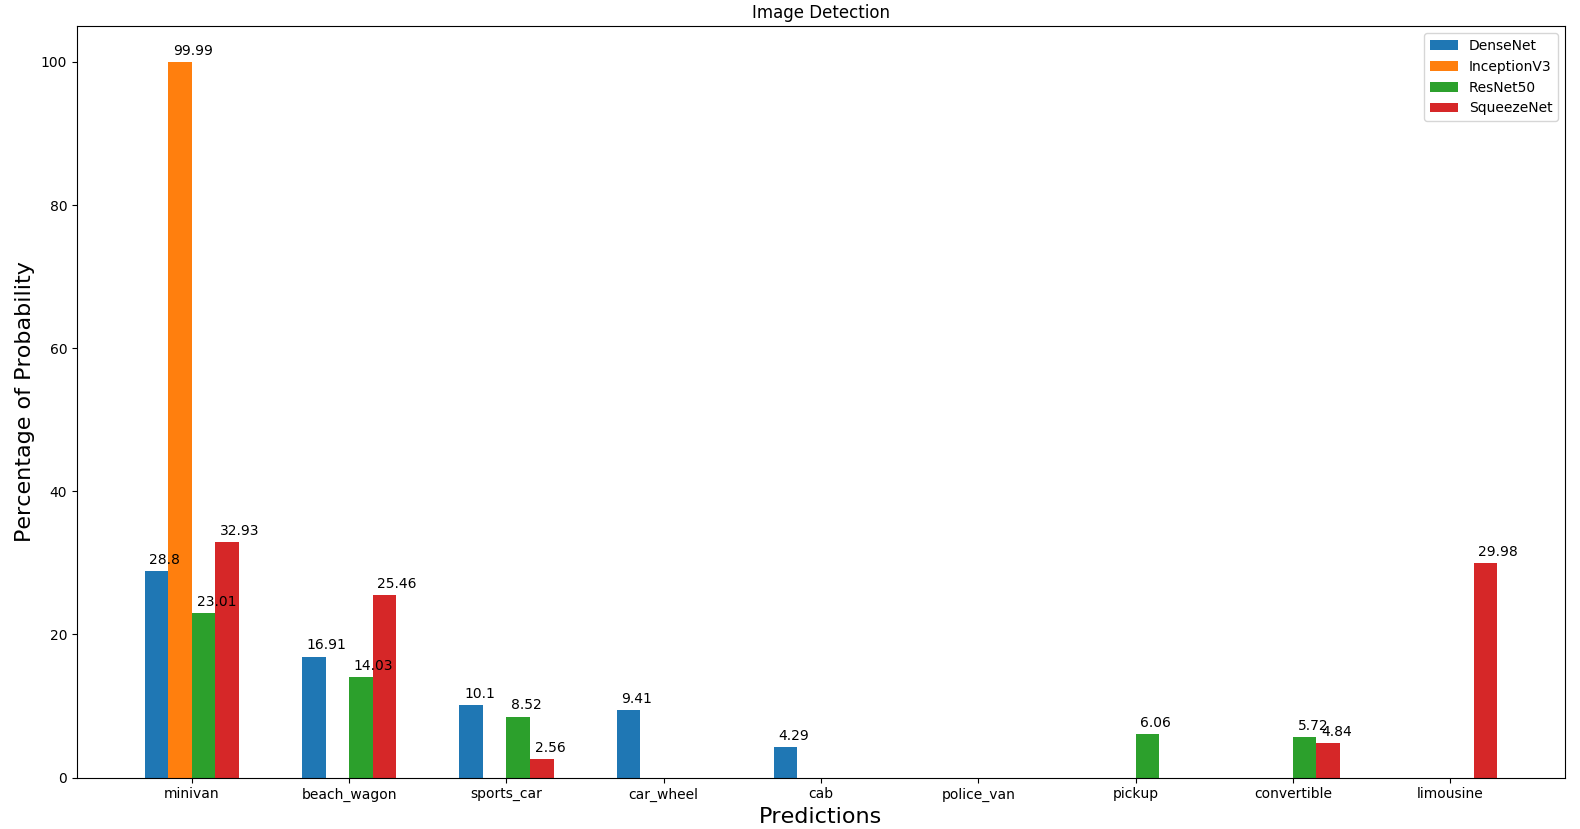
\includegraphics[scale = 0.37]{Sections/4InitialWork/4_images/run3_res.png}
        \caption{Results obtained.} 
    \end{figure}

    \newpage
    \subsection{Test Run Number 3}
    \par For the last run an image of an espresso was analysed by all 4 neural networks.
    \begin{figure}[htb]
        \centering
        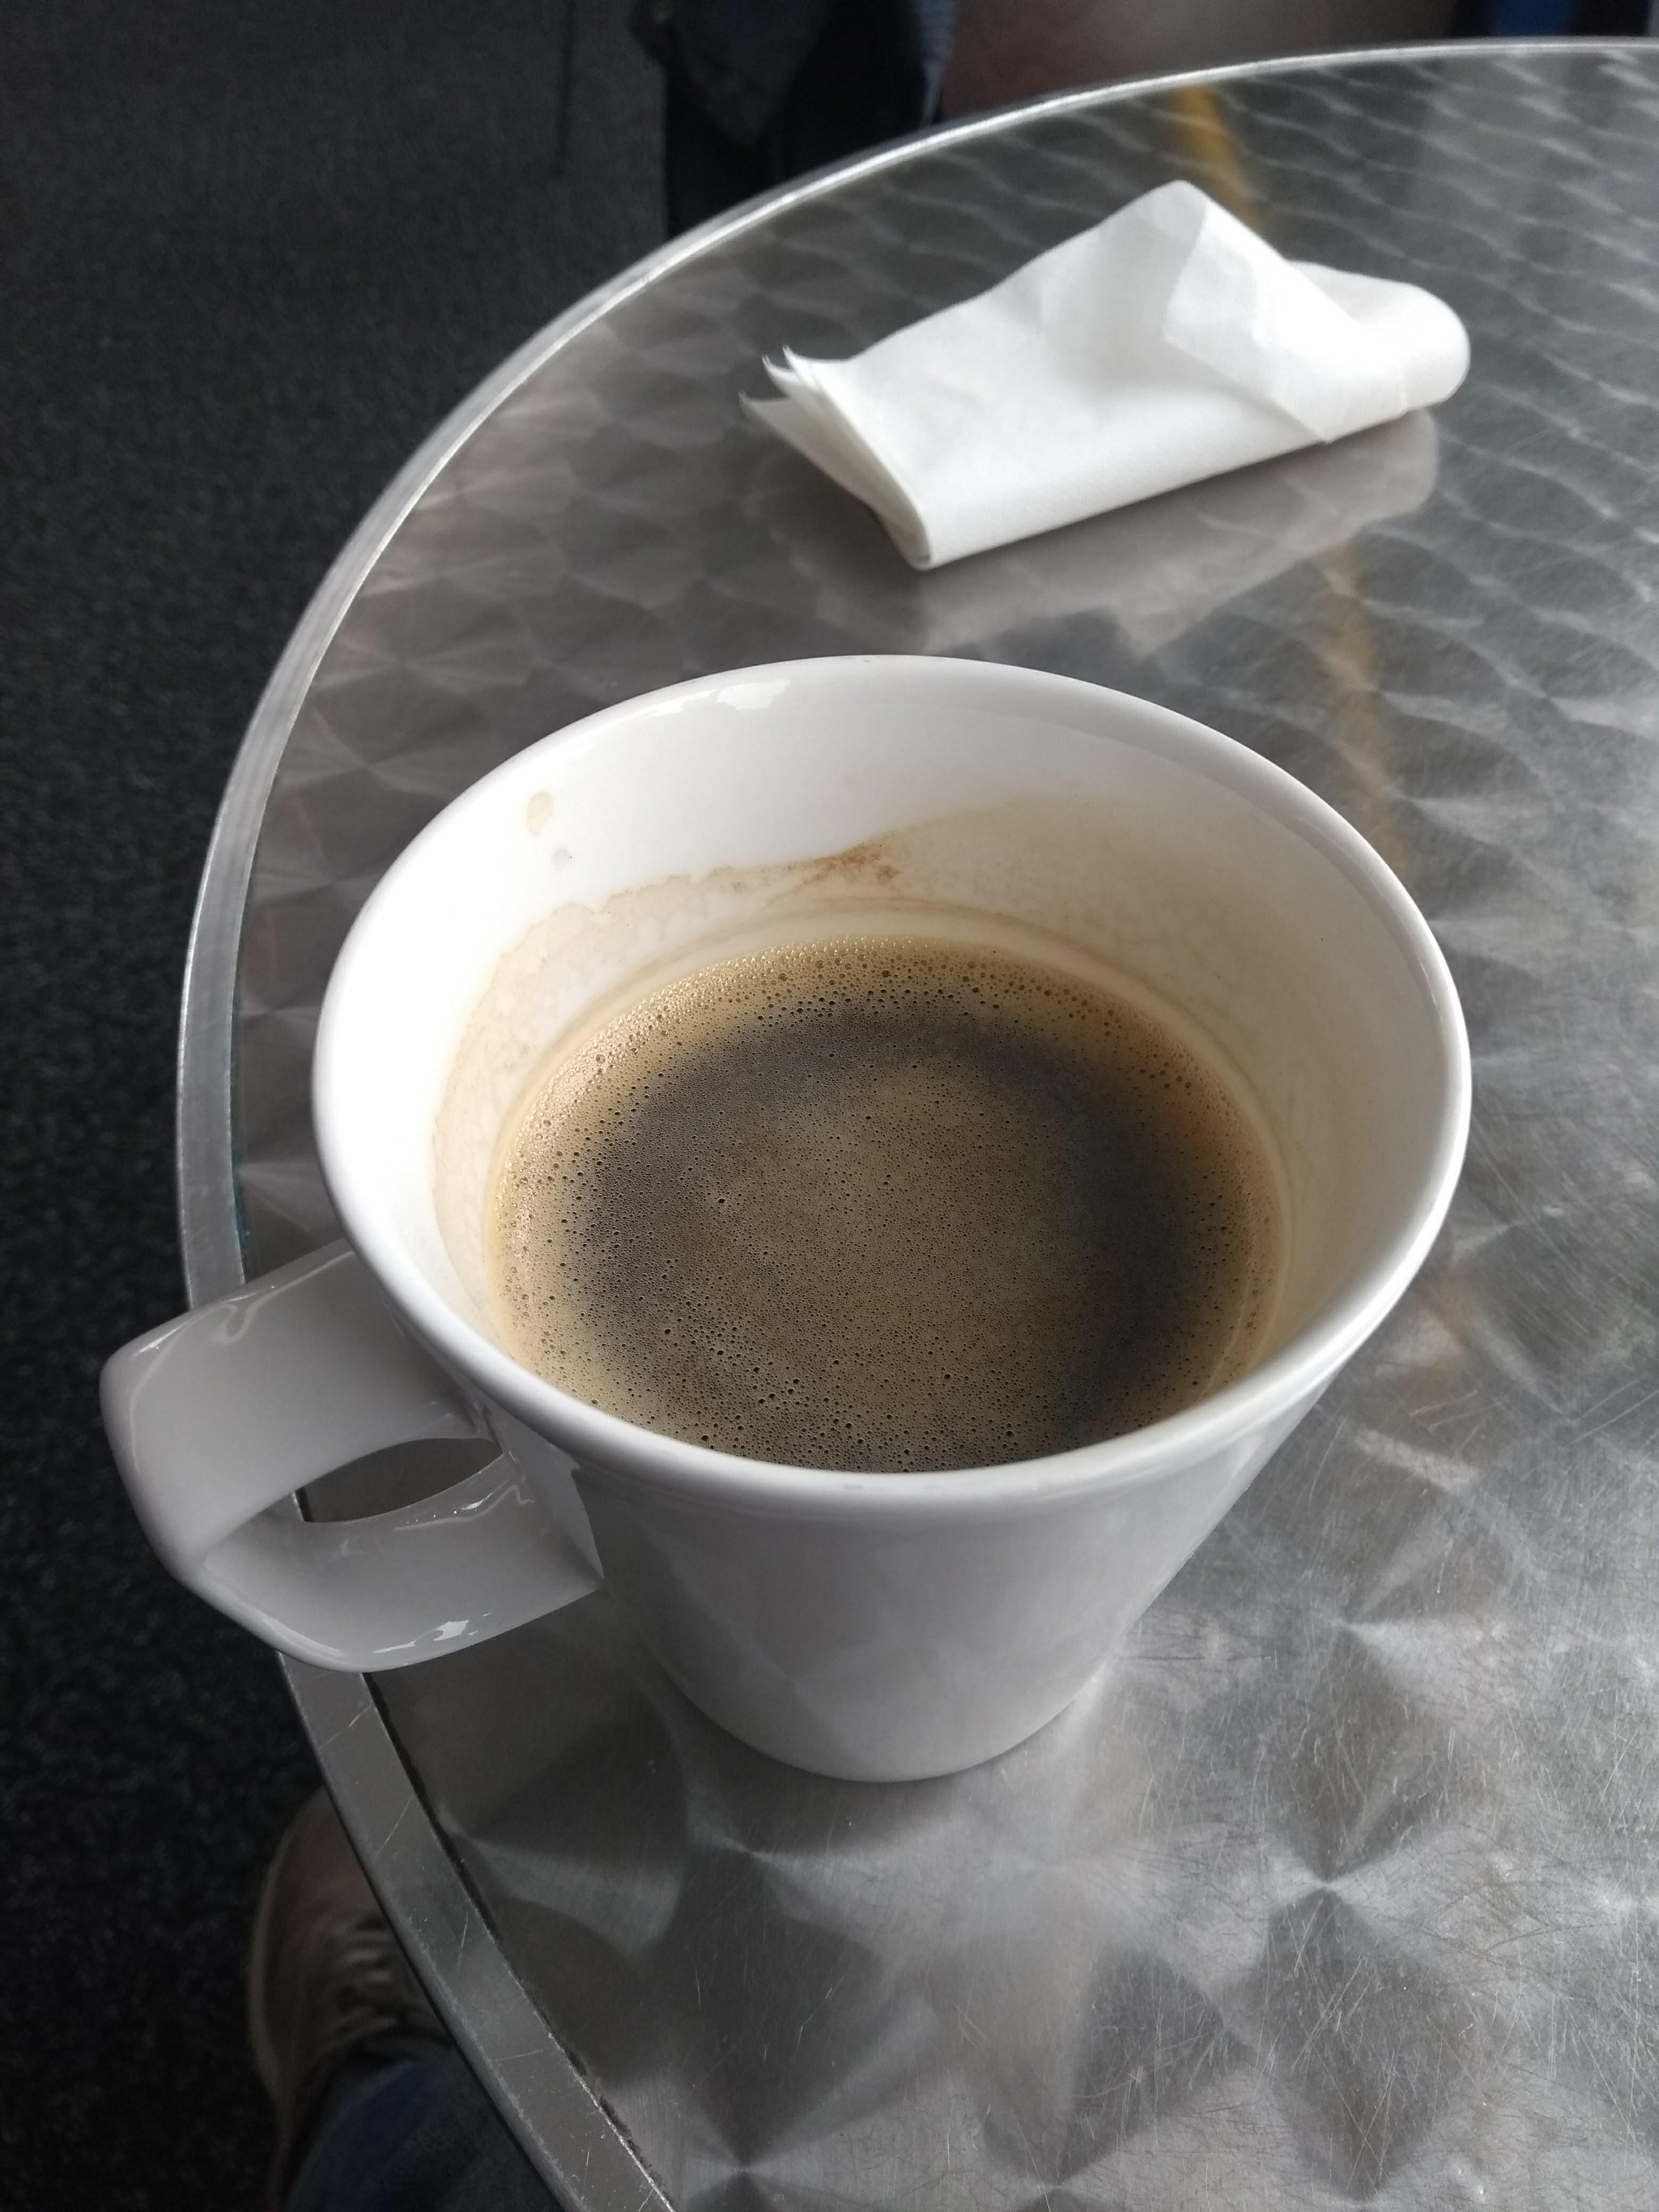
\includegraphics[scale = 0.04]{Sections/4InitialWork/4_images/run4_pic.jpg}
        \caption{Third picture to be analysed.} 
    \end{figure}
    \par The obtained results can be seen in the figure below
    \begin{figure}[htb]
        \centering
        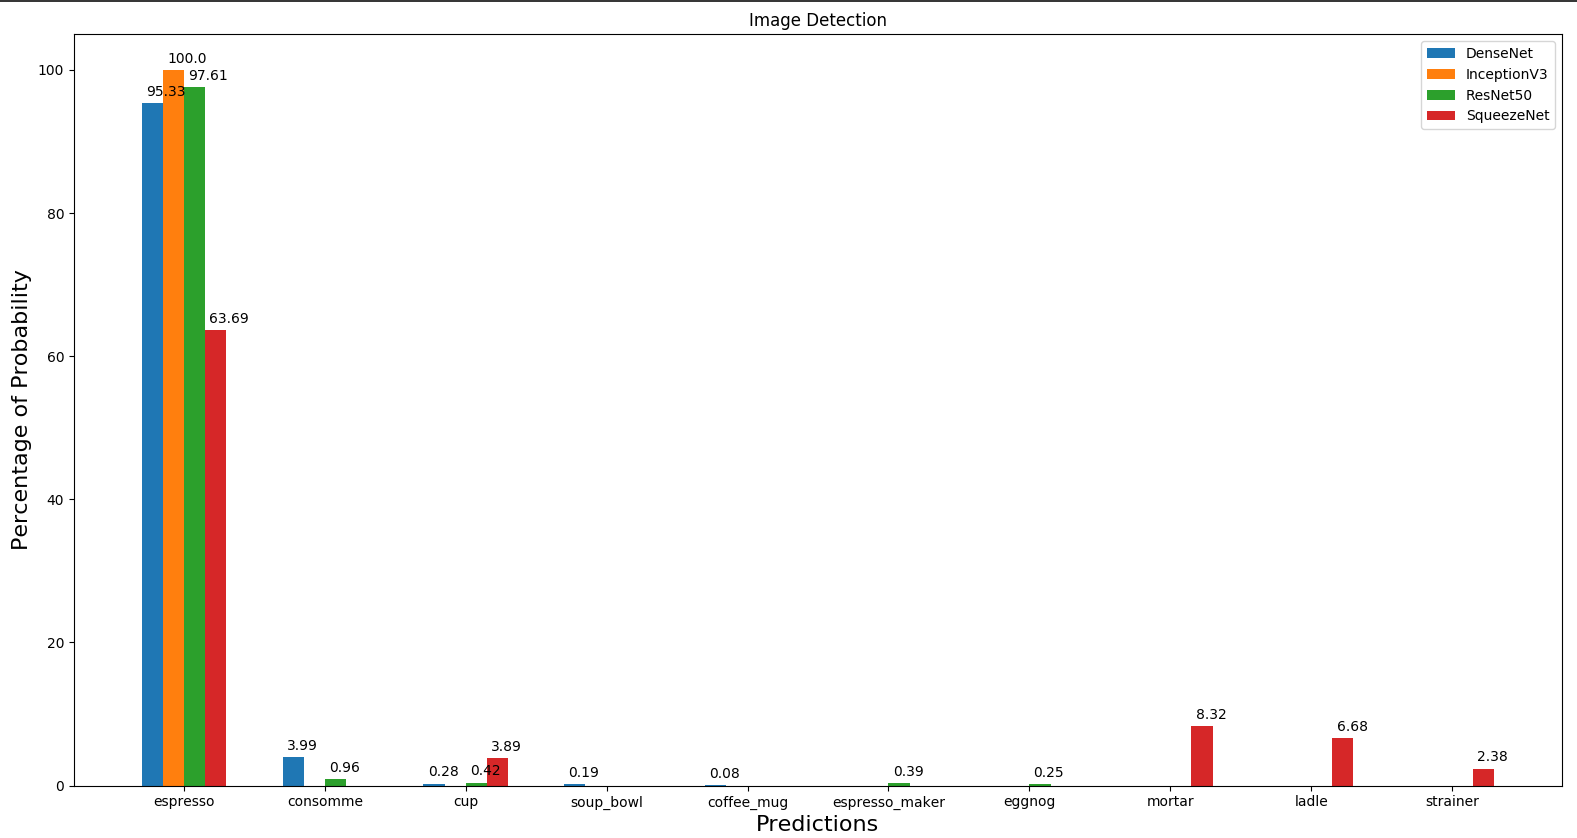
\includegraphics[scale = 0.37]{Sections/4InitialWork/4_images/run4_res.png}
        \caption{Results obtained.} 
    \end{figure}
    
    \newpage
    \subsection{Results analysis}
    \label{sec:results_image_rec}
    



 %%%%%%%%%%%%%%%%%%%%%%%%%%%%%%%%%%%%% OBJECT RECOGNITION   %%%%%%%%%%%%%%%%%%%%%%%%%%%%%%%%%%%%%
\newpage
\section{Object Recognition test runs}
\label{sec:object_test}

\par ImageAI provides 3 different models trained on the COCO dataset for object recognition that are able to identify up to 80 of the most common objects in everyday life. The models provide include RetinaNet, YOLOv3 and TinyYOLOv3. \cite{ImageAI}
\par The explanation on how these algorithms work is presented in chapter \ref{ch:computervision}. The analysis of the results is in section  \ref{sec:results_obj_rec}

    \subsection{Test Run Number 1}

    \begin{figure}[htb]
        \centering
        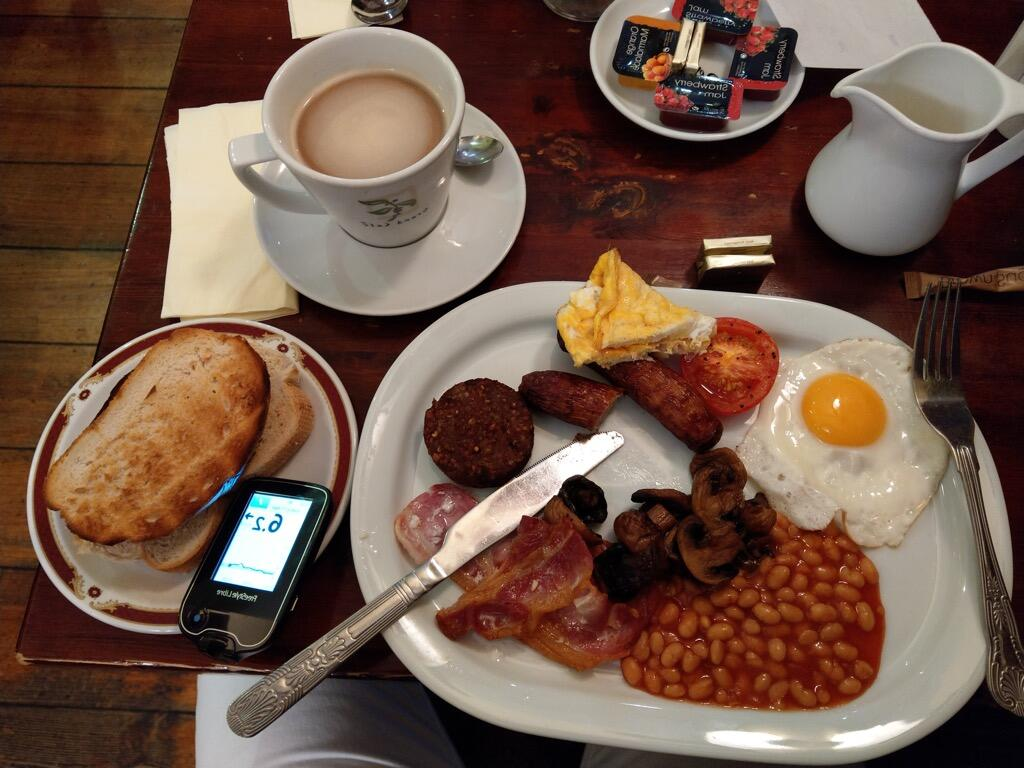
\includegraphics[scale = 0.20]{Sections/4InitialWork/4_images_obj_run1/photo.jpg}
        \caption{First picture to be analysed.} 
    \end{figure}

    \subsubsection{RetinaNet Results}

    \begin{figure}[htb]
        \centering
        \begin{minipage}[b]{0.44\textwidth}
          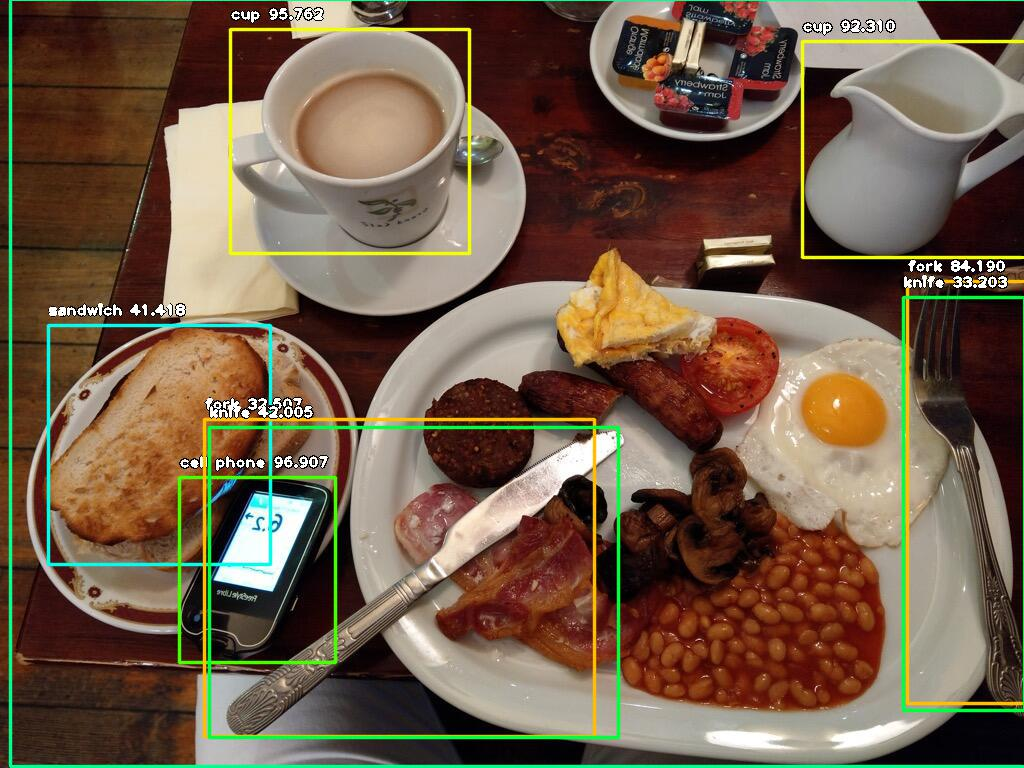
\includegraphics[width=\textwidth]{Sections/4InitialWork/4_images_obj_run1/retinaNet.jpg}
          \caption{RetinaNet Detections.}
        \end{minipage}
        \hfill
        \begin{minipage}[b]{0.50\textwidth}
          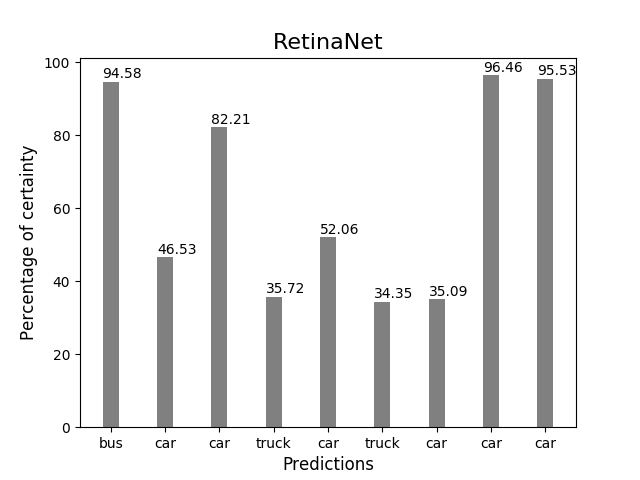
\includegraphics[width=\textwidth]{Sections/4InitialWork/4_images_obj_run1/retinaNet_graph.png}
          \caption{RetinaNet Detections.}
        \end{minipage}
      \end{figure}
    
    \newpage

    \subsubsection{Yolo Results}

    \begin{figure}[htb]
        \centering
        \begin{minipage}[b]{0.44\textwidth}
          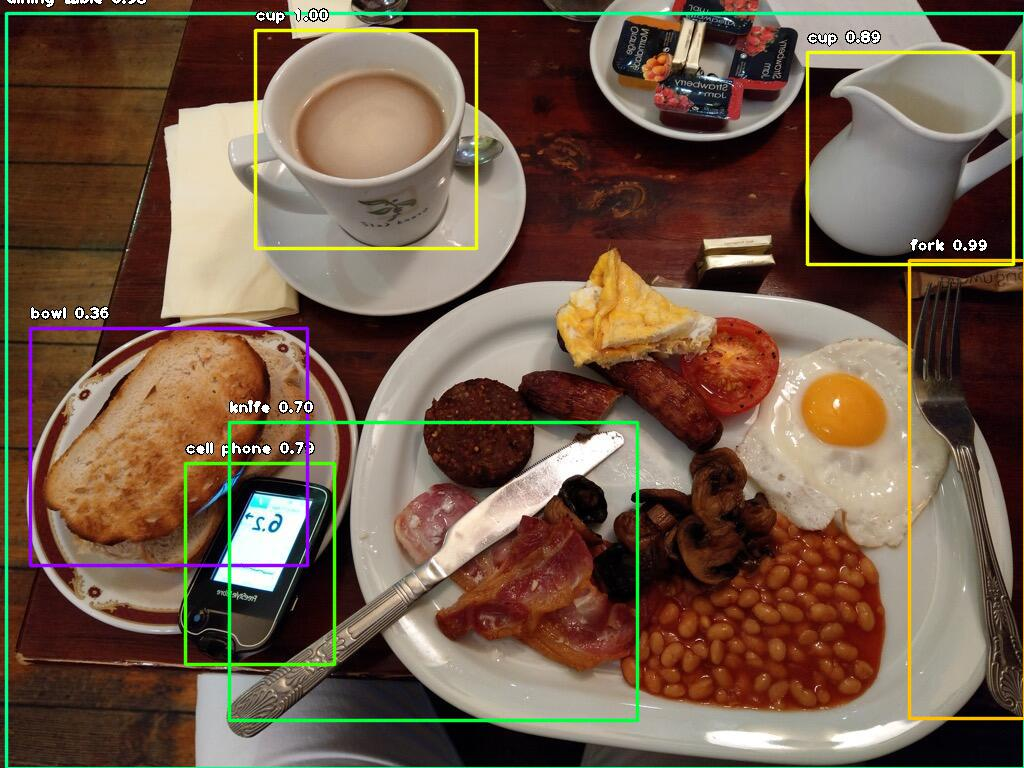
\includegraphics[width=\textwidth]{Sections/4InitialWork/4_images_obj_run1/yolo.jpg}
          \caption{YOLO Detections.}
        \end{minipage}
        \hfill
        \begin{minipage}[b]{0.50\textwidth}
          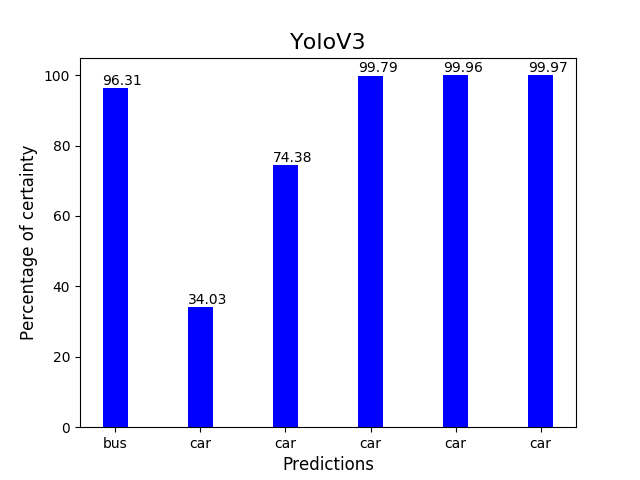
\includegraphics[width=\textwidth]{Sections/4InitialWork/4_images_obj_run1/yolo_graph.png}
          \caption{YOLO Detections.}
        \end{minipage}
      \end{figure}
    
      \subsubsection{TinyYolo Results}

    \begin{figure}[htb]
        \centering
        \begin{minipage}[b]{0.44\textwidth}
          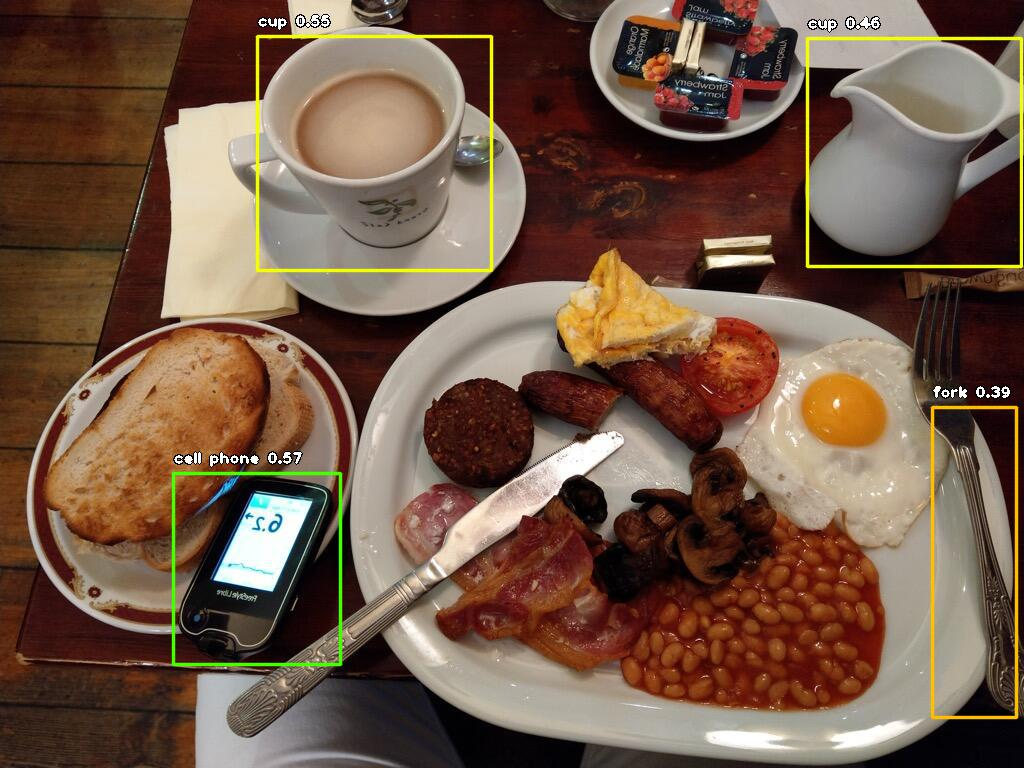
\includegraphics[width=\textwidth]{Sections/4InitialWork/4_images_obj_run1/yolo_tiny.jpg}
          \caption{TinyYolo Detections.}
        \end{minipage}
        \hfill
        \begin{minipage}[b]{0.50\textwidth}
          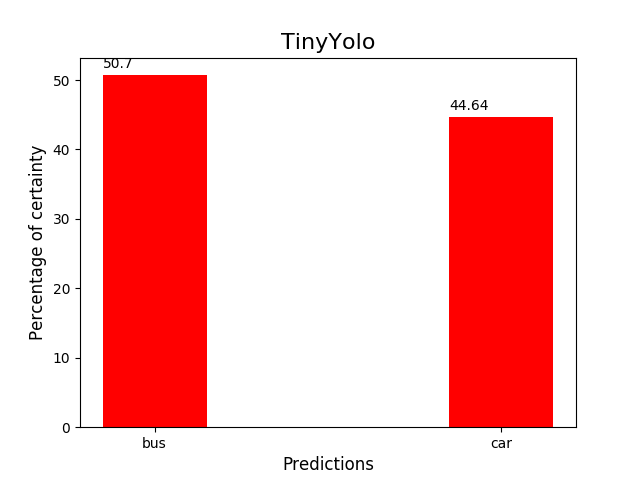
\includegraphics[width=\textwidth]{Sections/4InitialWork/4_images_obj_run1/yolo_tiny_graph.png}
          \caption{TinyYolo Detections.}
        \end{minipage}
      \end{figure}

    \newpage

 %%%%%%%%%%%%%%%%%%%%%%%%%%%%%%%%%%%%% run2   %%%%%%%%%%%%%%%%%%%%%%%%%%%%%%%%%%%%%
    \subsection{Test Run Number 2}

    \begin{figure}[htb]
        \centering
        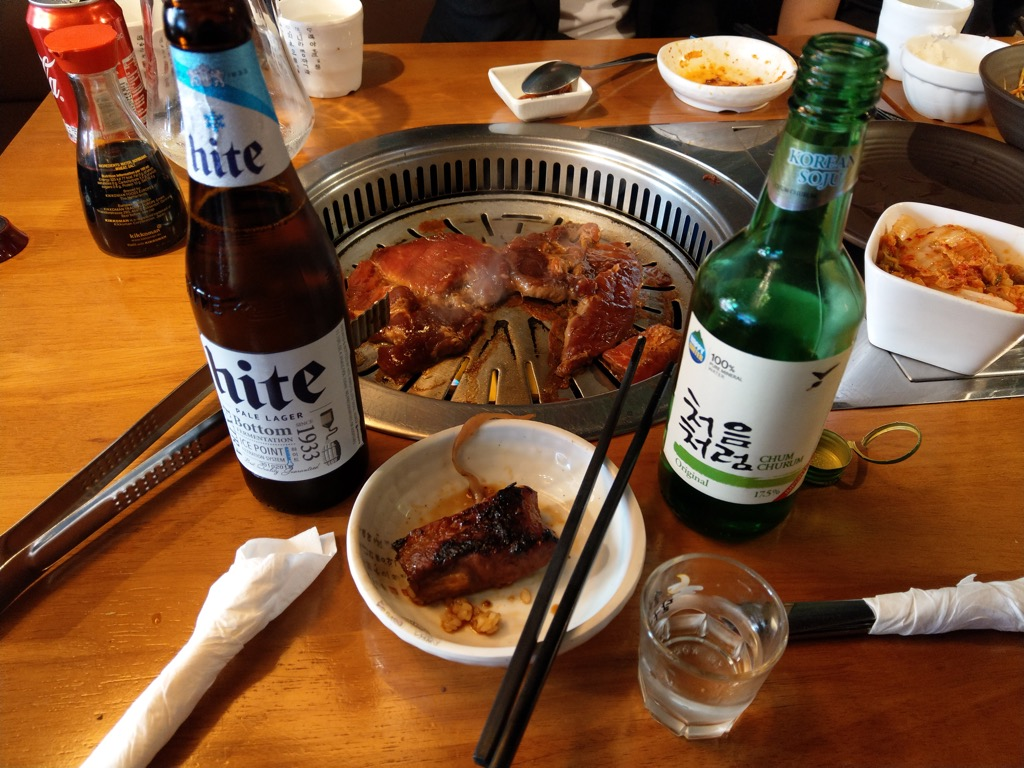
\includegraphics[scale = 0.20]{Sections/4InitialWork/4_images_obj_run2/photo.jpg}
        \caption{Second picture to be analysed.} 
    \end{figure}

    \subsubsection{RetinaNet run 2 results}

    \begin{figure}[htb]
        \centering
        \begin{minipage}[b]{0.44\textwidth}
          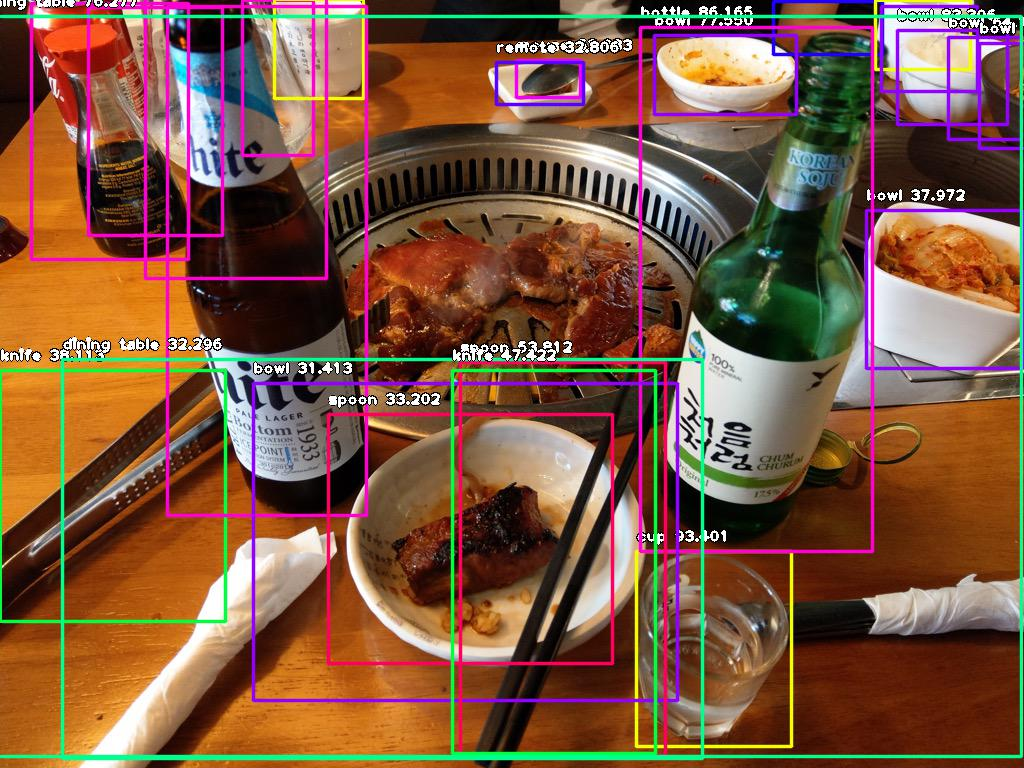
\includegraphics[width=\textwidth]{Sections/4InitialWork/4_images_obj_run2/retinaNet.jpg}
          \caption{RetinaNet Detections.}
        \end{minipage}
        \hfill
        \begin{minipage}[b]{0.50\textwidth}
          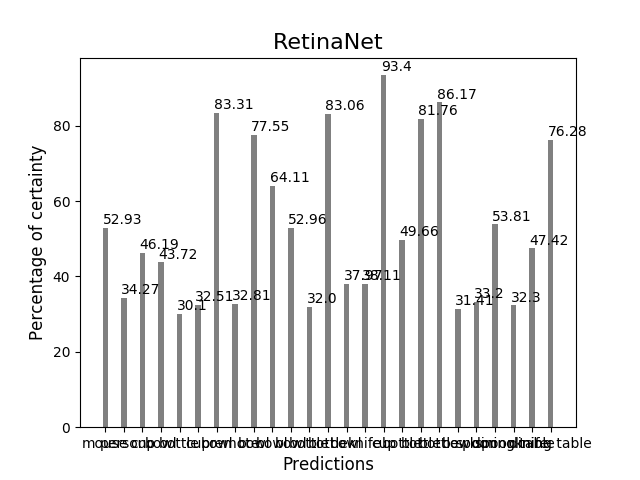
\includegraphics[width=\textwidth]{Sections/4InitialWork/4_images_obj_run2/retinaNet_graph.png}
          \caption{RetinaNet Detections.}
        \end{minipage}
      \end{figure}
    
    \newpage

    \subsubsection{Yolo run 2 results}

    \begin{figure}[htb]
        \centering
        \begin{minipage}[b]{0.44\textwidth}
          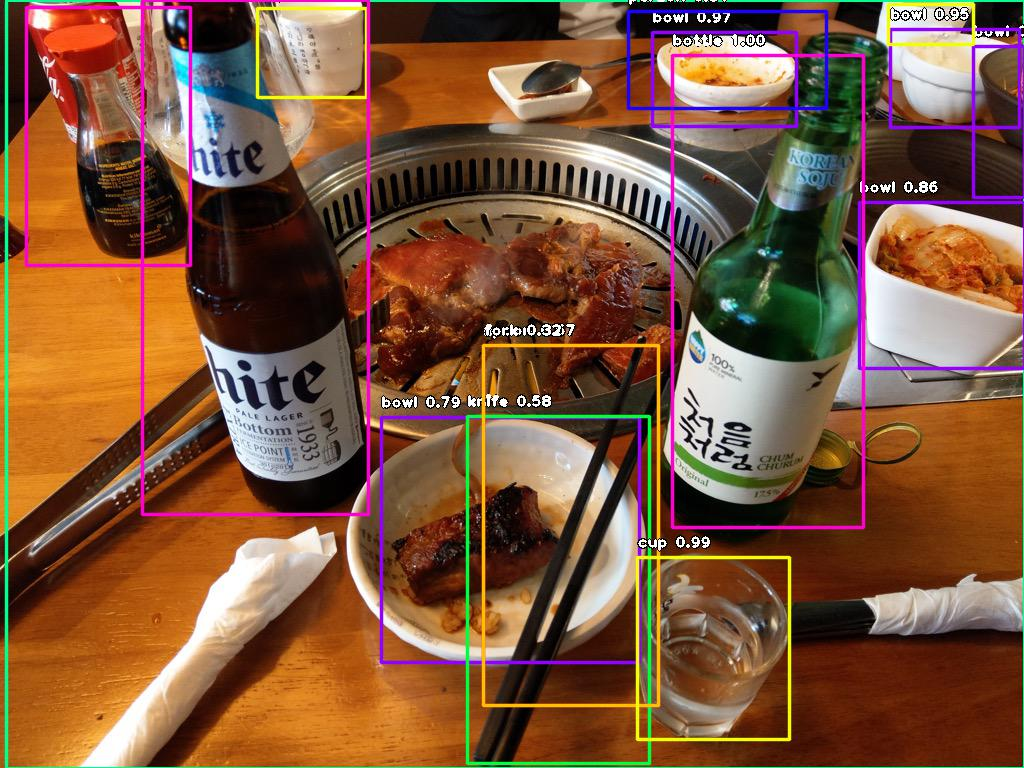
\includegraphics[width=\textwidth]{Sections/4InitialWork/4_images_obj_run2/yolo.jpg}
          \caption{YOLO Detections.}
        \end{minipage}
        \hfill
        \begin{minipage}[b]{0.50\textwidth}
          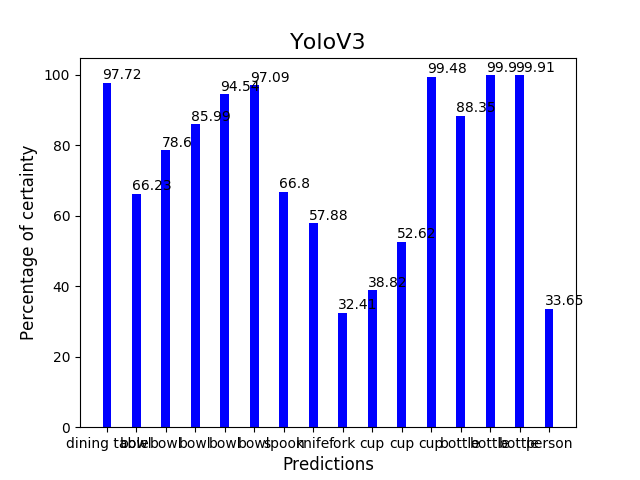
\includegraphics[width=\textwidth]{Sections/4InitialWork/4_images_obj_run2/yolo_graph.png}
          \caption{YOLO Detections.}
        \end{minipage}
      \end{figure}
    
      \subsubsection{TinyYolo run 2 results}

    \begin{figure}[htb]
        \centering
        \begin{minipage}[b]{0.44\textwidth}
          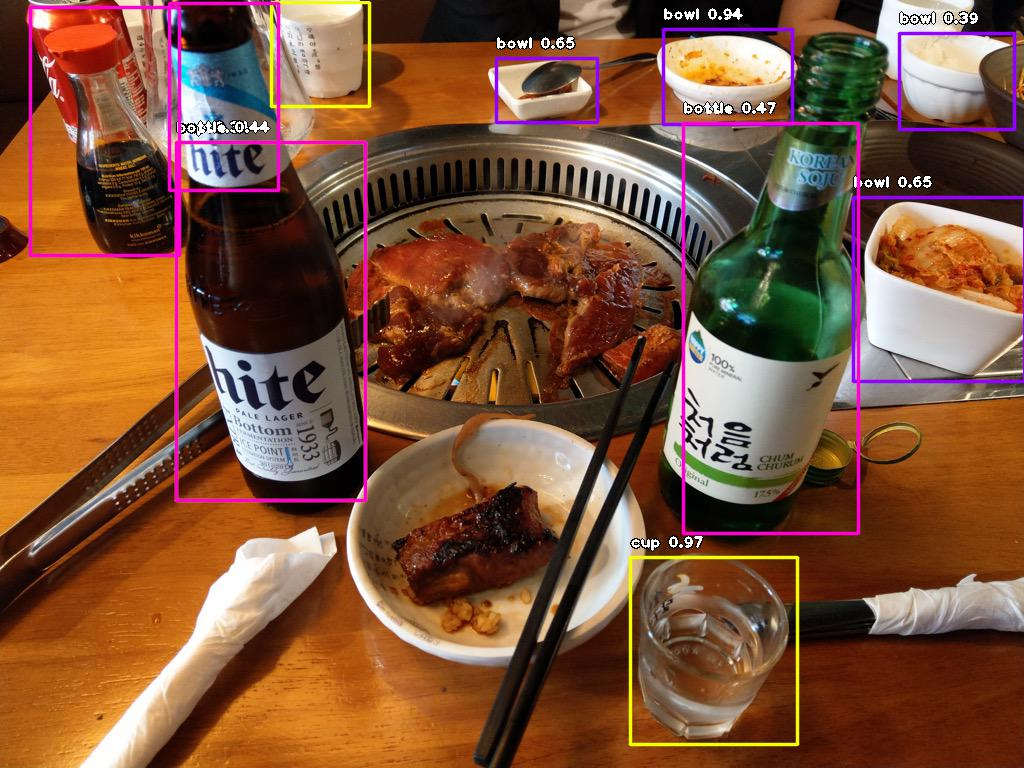
\includegraphics[width=\textwidth]{Sections/4InitialWork/4_images_obj_run2/yolo_tiny.jpg}
          \caption{TinyYolo Detections.}
        \end{minipage}
        \hfill
        \begin{minipage}[b]{0.50\textwidth}
          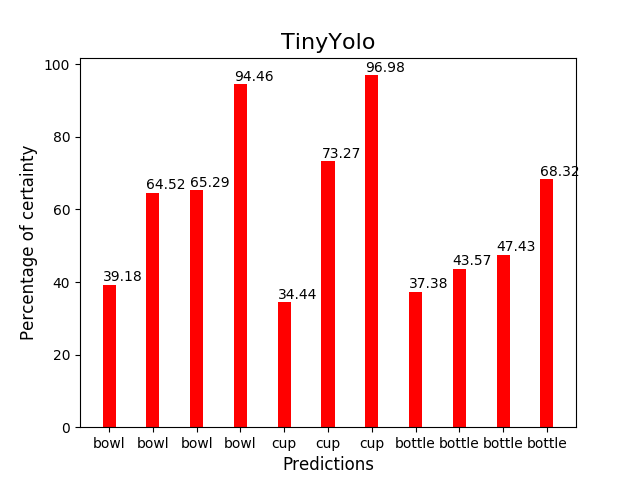
\includegraphics[width=\textwidth]{Sections/4InitialWork/4_images_obj_run2/yolo_tiny_graph.png}
          \caption{TinyYolo Detections.}
        \end{minipage}
      \end{figure}

    \newpage


 %%%%%%%%%%%%%%%%%%%%%%%%%%%%%%%%%%%%% run3 %%%%%%%%%%%%%%%%%%%%%%%%%%%%%%%%%%%%%
    \subsection{Test Run Number 3}

    \begin{figure}[htb]
        \centering
        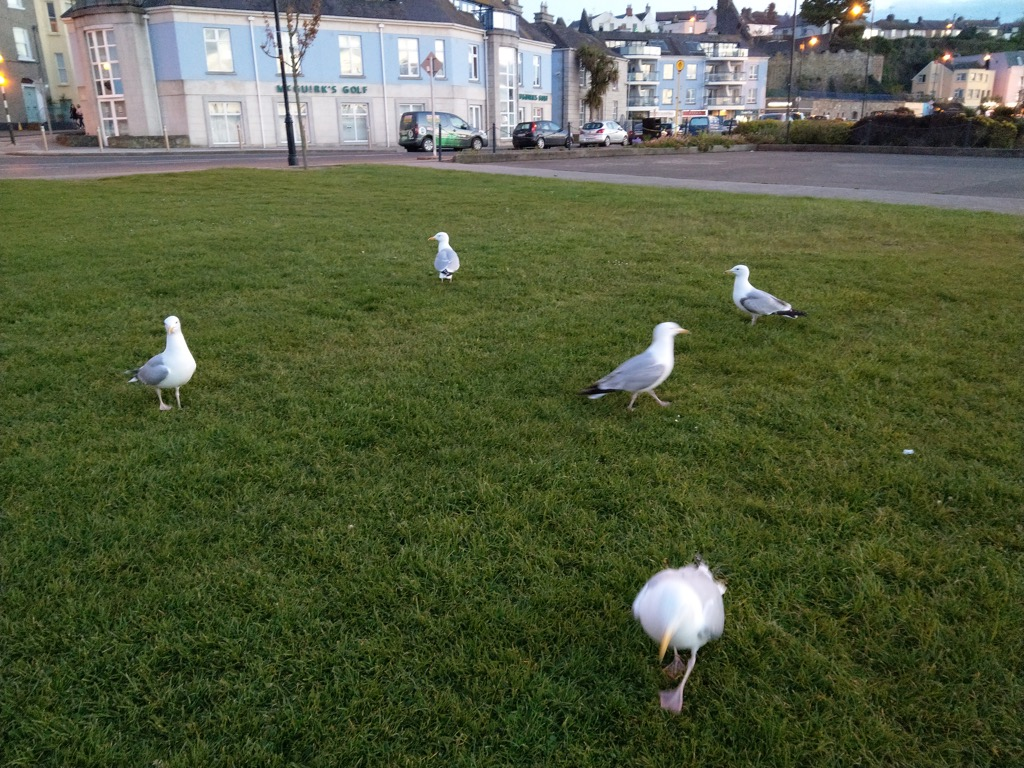
\includegraphics[scale = 0.20]{Sections/4InitialWork/4_images_obj_run3/photo.jpg}
        \caption{Third picture to be analysed.} 
    \end{figure}

    \subsubsection{RetinaNet Results}

    \begin{figure}[htb]
        \centering
        \begin{minipage}[b]{0.44\textwidth}
          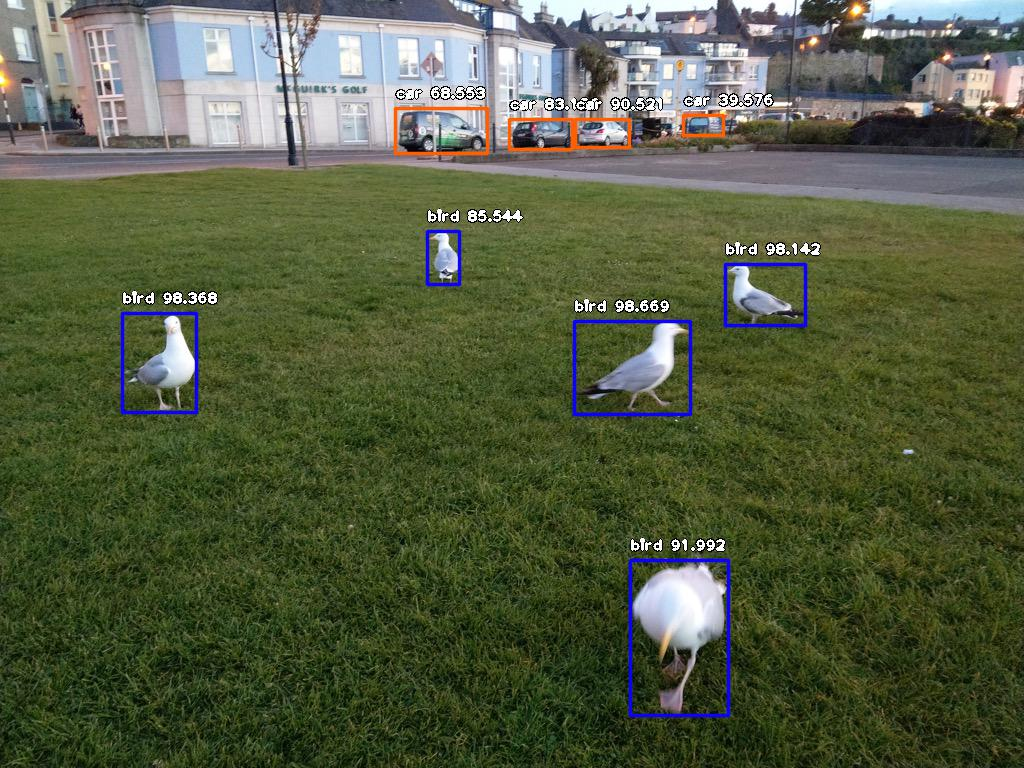
\includegraphics[width=\textwidth]{Sections/4InitialWork/4_images_obj_run3/retinaNet.jpg}
          \caption{RetinaNet Detections.}
        \end{minipage}
        \hfill
        \begin{minipage}[b]{0.50\textwidth}
          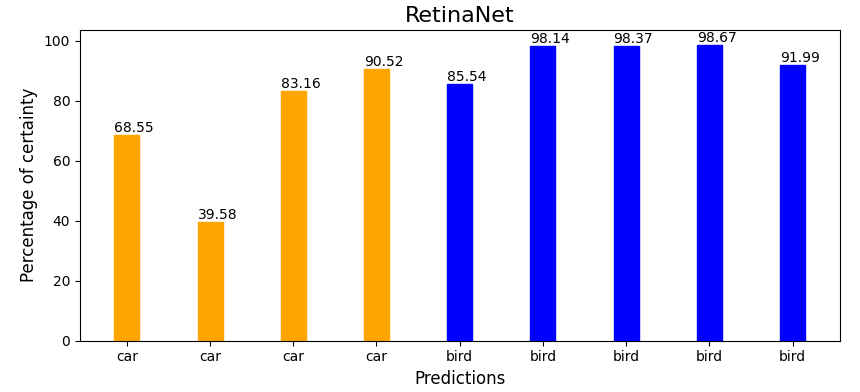
\includegraphics[width=\textwidth]{Sections/4InitialWork/4_images_obj_run3/retinaNet_graph.png}
          \caption{RetinaNet Detections.}
        \end{minipage}
      \end{figure}
    
    \newpage

    \subsubsection{YOLO Results}
    
    \begin{figure}[htb]
        \centering
        \begin{minipage}[b]{0.44\textwidth}
          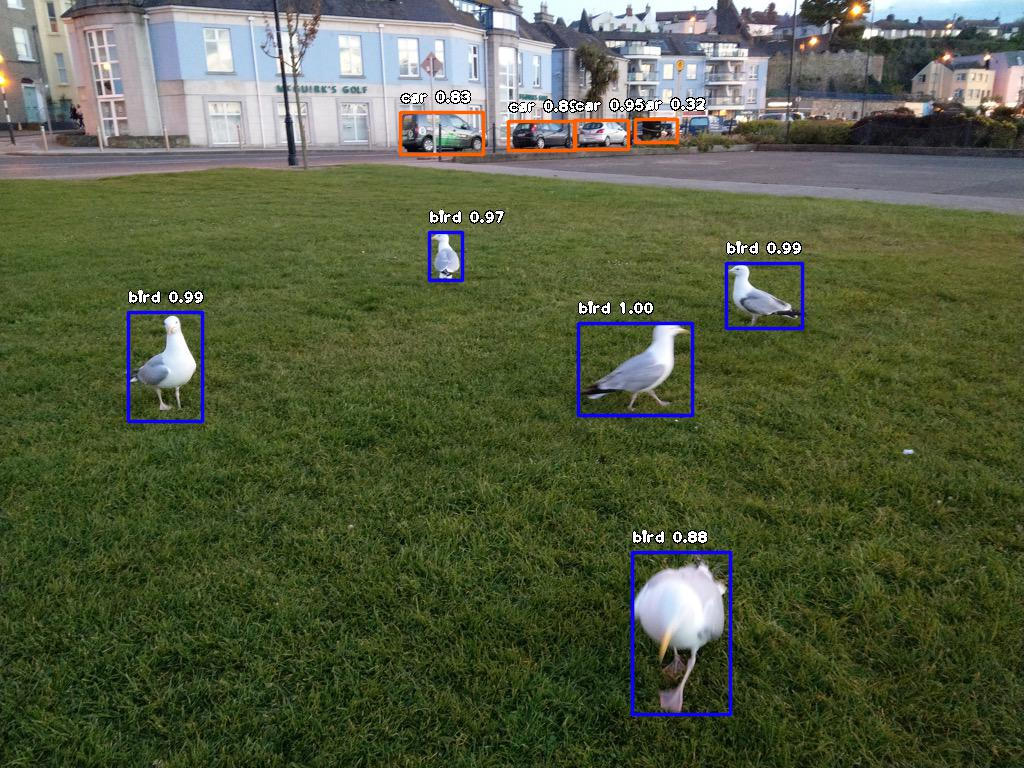
\includegraphics[width=\textwidth]{Sections/4InitialWork/4_images_obj_run3/yolo.jpg}
          \caption{YOLO Detections.}
        \end{minipage}
        \hfill
        \begin{minipage}[b]{0.50\textwidth}
          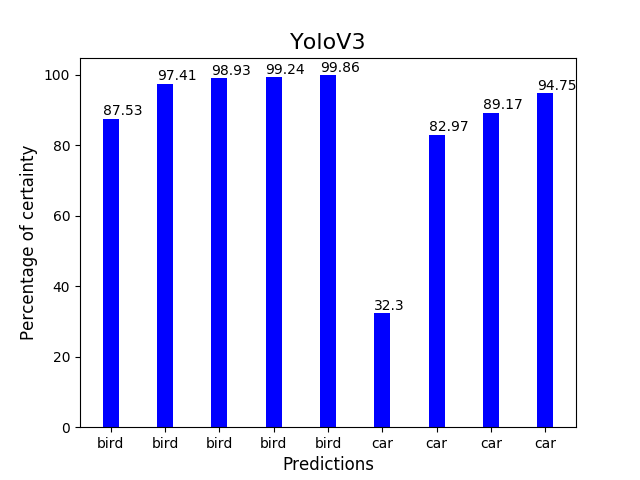
\includegraphics[width=\textwidth]{Sections/4InitialWork/4_images_obj_run3/yolo_graph.png}
          \caption{YOLO Detections.}
        \end{minipage}
      \end{figure}
    
      \subsubsection{TinyYOLO Results}

    \begin{figure}[htb]
        \centering
        \begin{minipage}[b]{0.44\textwidth}
          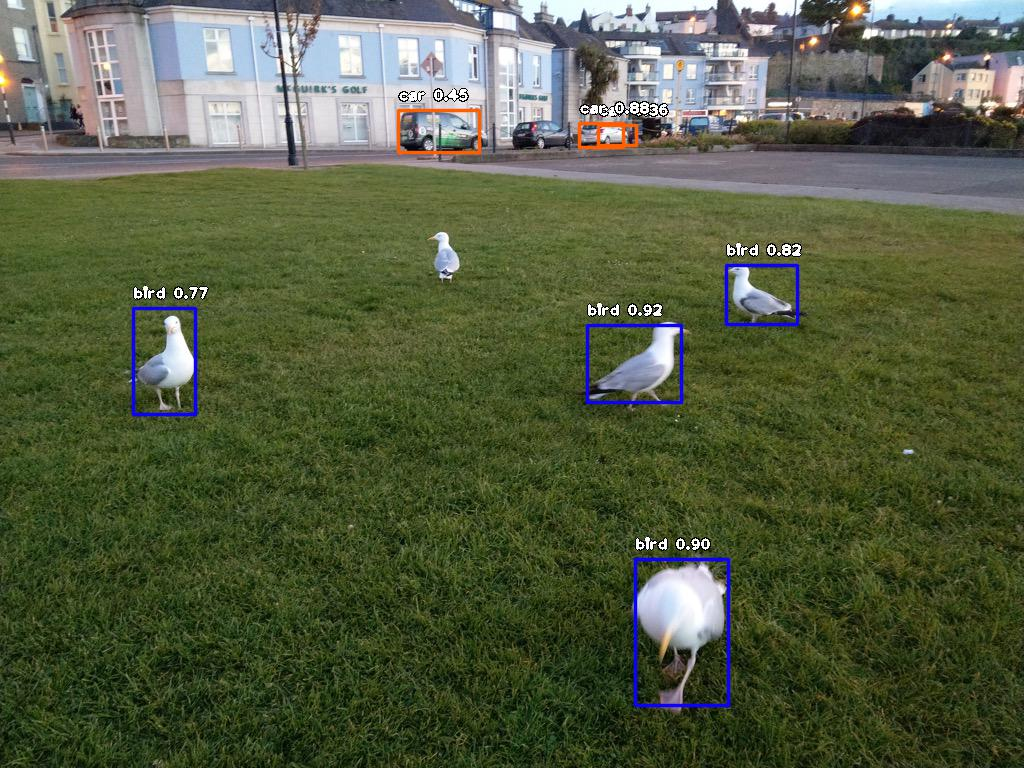
\includegraphics[width=\textwidth]{Sections/4InitialWork/4_images_obj_run3/yolo_tiny.jpg}
          \caption{TinyYolo Detections.}
        \end{minipage}
        \hfill
        \begin{minipage}[b]{0.50\textwidth}
          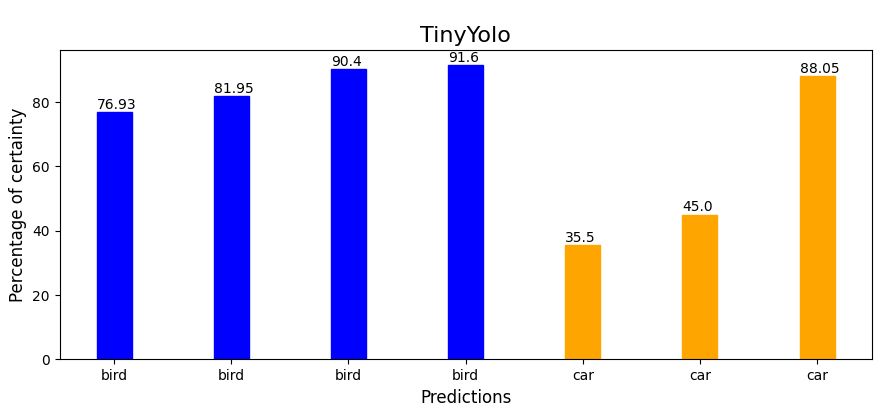
\includegraphics[width=\textwidth]{Sections/4InitialWork/4_images_obj_run3/yolo_tiny_graph.png}
          \caption{TinyYolo Detections.}
        \end{minipage}
      \end{figure}

    \newpage
    \subsection{Results analysis}

    \label{sec:results_obj_rec}

